\documentclass[10pt,a4paper]{article}
\usepackage[T1]{fontenc}
\usepackage[utf8]{inputenc}
\usepackage{lmodern}
\usepackage[margin=2.2cm]{geometry}
\usepackage{amsmath,amssymb}
\usepackage{booktabs}
\usepackage{longtable}
\usepackage{graphicx}
\usepackage{float}
\usepackage{xcolor}
\usepackage[font=small,labelfont=bf]{caption}
\usepackage{microtype}
\usepackage{enumitem}
\usepackage[colorlinks=true,linkcolor=blue!50!black,citecolor=blue!50!black,urlcolor=blue!50!black]{hyperref}
\setlist{itemsep=1pt,topsep=3pt}
\newcommand{\nNStudiesHL}{25}
\newcommand{\nTHalf}{5.20}
\newcommand{\nTHalfQone}{4.3}
\newcommand{\nTHalfQthree}{5.6}
\newcommand{\nTHalfMin}{3.4}
\newcommand{\nTHalfMax}{7.1}
\newcommand{\nKe}{0.1333}
\newcommand{\nKa}{4.42}
\newcommand{\nTmaxMed}{49}
\newcommand{\nTmaxModel}{49}
\newcommand{\nVkg}{0.669}
\newcommand{\nCLmodel}{1.49}
\newcommand{\nPeakFrac}{0.897}
\newcommand{\nRatioMed}{0.81}
\newcommand{\nRatioMin}{0.67}
\newcommand{\nRatioMax}{0.92}
\newcommand{\nWithin}{4}
\newcommand{\nNValid}{8}
\newcommand{\nPopPeakRatio}{1.01}
\newcommand{\nRatioPopMed}{0.81}
\newcommand{\nRatioPopMin}{0.68}
\newcommand{\nRatioPopMax}{0.93}
\newcommand{\nWithinPop}{5}
\newcommand{\nLandoltHalf}{5.9}
\newcommand{\nGCoffee}{34}
\newcommand{\nGPrew}{39}
\newcommand{\nLandoltMg}{37}
\newcommand{\nDrakeMg}{185}
\newcommand{\nRefMg}{36}
\newcommand{\nRefMgKg}{0.52}
\newcommand{\nRefConc}{0.78}
\newcommand{\nDayBed}{111}
\newcommand{\nDayBedLo}{66}
\newcommand{\nDayBedHi}{172}
\newcommand{\nTHalfTen}{3.4}
\newcommand{\nTHalfNinety}{8.4}
\newcommand{\nTRefOneFifty}{10.9}
\newcommand{\nCupMg}{100}
\newcommand{\nSmEmax}{1.05}
\newcommand{\nSmEcfifty}{10.3}
\newcommand{\nSmTdeind}{38.6}
\newcommand{\nSmMten}{1.52}
\newcommand{\nSmMtwenty}{1.69}
\newcommand{\nSmMforty}{1.84}
\newcommand{\nSmMfive}{1.34}
\newcommand{\nSmThalfTen}{3.4}
\newcommand{\nSmThalfTwenty}{3.1}
\newcommand{\nSmThalfFive}{3.9}
\newcommand{\nSmScM}{1.69}
\newcommand{\nSmScMtwo}{1.40}
\newcommand{\nSmScMseven}{1.05}
\newcommand{\nSmMaxErr}{0.05}
\newcommand{\nSmBedSmoke}{26}
\newcommand{\nSmBedBase}{68}
\newcommand{\nSmWindow}{28}
\newcommand{\nSmStartAvg}{7}

\newcommand{\halflifetable}{%
Parsons 1978 & \emph{Clin Pharmacol Ther} & non-smokers & 6.00 & 657717\\
Statland 1980 & \emph{Am J Clin Pathol} & healthy subjects & 5.70 & 7361718\\
Desmond 1980 & \emph{Dig Dis Sci} & healthy controls & 5.20 & 7371463\\
Knutti 1981 & \emph{Eur J Clin Pharmacol} & men and non-pregnant women (saliva) & 3.40 & 7341280\\
Newton 1981 & \emph{Eur J Clin Pharmacol} & 50 mg dose & 4.25 & 7333346\\
Mitchell 1983 & \emph{J Lab Clin Med} & baseline & 4.03 & 6854123\\
Renner 1984 & \emph{Hepatology} & normal volunteers & 3.80 & 6420303\\
Whitsett 1984 & \emph{Am J Cardiol} & non-smokers & 5.10 & 6702647\\
Abernethy 1985 & \emph{Eur J Clin Pharmacol} & women, no oral contraceptives & 5.37 & 4029248\\
Lelo 1986 & \emph{Br J Clin Pharmacol} & men & 4.10 & 3756065\\
Bruce 1986 & \emph{Br J Clin Pharmacol} & healthy (approximate) & 5.00 & 3741730\\
Mays 1987 & \emph{Clin Pharmacol Ther} & baseline & 5.60 & 3690940\\
Healy 1989 & \emph{Antimicrob Agents Chemother} & baseline & 5.20 & 2729942\\
Wahlländer 1989 & \emph{Eur J Clin Pharmacol} & controls & 5.80 & 2612543\\
Collomp 1991 & \emph{Eur J Clin Pharmacol} & at rest & 3.99 & 2060565\\
Mahr 1992 & \emph{Clin Pharmacokinet} & placebo phase & 4.50 & 1319876\\
Kamimori 1995 & \emph{Eur J Clin Pharmacol} & sea level & 6.70 & 7589033\\
Soto 1997 & \emph{J Clin Pharm Ther} & baseline & 5.30 & 9447474\\
Forsyth 2000 & \emph{Br J Clin Pharmacol} & healthy controls (saliva) & 5.75 & 11012552\\
Haller 2002 & \emph{Clin Pharmacol Ther} & no oral contraceptives & 5.60 & 12087345\\
Haller 2004 & \emph{Clin Pharmacol Ther} & men & 5.00 & 15060505\\
Culm-Merdek 2005 & \emph{Br J Clin Pharmacol} & placebo phase & 4.90 & 16236038\\
Seng 2009 & \emph{J Clin Pharm Ther} & non-smokers (population PK) & 4.30 & 19125908\\
White 2016 & \emph{Clin Toxicol} & men and women, incl. OC users & 7.08 & 27100333\\
Thai 2021 & \emph{Clin Pharmacol Drug Dev} & placebo phase & 5.40 & 33951339\\
}
\newcommand{\validtable}{%
Blanchard 1983 (solution, 5 mg/kg) & 10.00 & 6.71 & 0.67\\
White 2016 hot coffee (160 mg, 74 kg) & 3.74 & 2.90 & 0.78\\
White 2016 cold coffee 2 min & 3.64 & 2.90 & 0.80\\
White 2016 cold coffee 20 min & 3.56 & 2.90 & 0.81\\
White 2016 energy drink 2 min & 3.36 & 2.90 & 0.86\\
White 2016 energy drink 20 min & 3.14 & 2.90 & 0.92\\
Landolt 1995 peak (200 mg, saliva, 70 kg assumed) & 4.46 & 3.80 & 0.85\\
Landolt 1995 at 23:00, 15.8 h later & 0.79 & 0.53 & 0.68\\
}
\newcommand{\tmaxtable}{%
Blanchard 1983, solution 5 mg/kg & 30\\
Liguori 1997, coffee 400 mg (saliva) & 42\\
Liguori 1997, cola 400 mg (saliva) & 39\\
Abernethy 1985, 162 mg (controls) & 47\\
White 2016, hot coffee over 20 min & 49\\
White 2016, cold coffee over 2 min & 61\\
White 2016, cold coffee over 20 min & 54\\
White 2016, energy drink over 2 min & 69\\
White 2016, energy drink over 20 min & 72\\
}
\newcommand{\cltable}{%
Lelo 1986 & 2.07\\
Abernethy 1985 (controls) & 1.75\\
White 2016 (5 arms) & 1.32\\
Wahlländer 1989 (controls) & 1.34\\
Newton 1981 & 0.98\\
Faber 2004 (after quitting smoking) & 1.53\\
Seng 2009 (114 mL/min, 65 kg) & 1.75\\
}
\newcommand{\smoketable}{%
Parsons 1978 & 13 smokers vs 13 non-smokers & 1.65 & 1.69 & 1.03 & cigarettes/day not given; 20 assumed\\
Joeres 1988 & 8 smokers vs 15 non-smokers & 1.78 & 1.69 & 0.95 & 20 assumed\\
Seng 2009 & population PK, 59 men & 1.96 & 1.69 & 0.86 & 20 assumed\\
Faber 2004 & 12 heavy smokers, before vs 13 d after quitting & 1.61 & 1.74 & 1.08 & $\geq$20/day\\
Joeres 1988 & 7 smokers, before vs 3 weeks after quitting & 1.53 & 1.69 & 1.11 & 20 assumed\\
Benowitz 2003 & 12 smokers, smoking vs 7 d of air & 1.33 & 1.64 & 1.23 & 20 assumed\\
Brown 1988 & 9 smokers, 24-h AUC after 4 d abstinence & 1.46 & 1.51 & 1.03 & AUC ratio; 20 assumed\\
}
\newcommand{\siptable}{%
all at once & 135 & 49 & 134 & 69.5 & 46.6 & 31.2\\
15 min & 134 & 57 & 134 & 70.7 & 47.4 & 31.8\\
30 min & 134 & 67 & 133 & 71.9 & 48.2 & 32.3\\
60 min & 132 & 89 & 110 & 74.4 & 49.8 & 33.4\\
120 min & 126 & 140 & 55 & 79.7 & 53.4 & 35.8\\
}
\newcommand{\sipwhitetable}{%
White 2016, cold coffee / energy drink over 2 min & 62 / 70 & 50\\
White 2016, hot / cold coffee / energy drink over 20 min & 59 / 64 / 82 & 60\\
}
\newcommand{\voltable}{%
Lelo 1986 & 0.68\\
Abernethy 1985 & 0.75\\
White 2016 & 0.66\\
Seng 2009 (42 L, CL 114 mL/min, assumed 65 kg) & 0.65\\
}

\newcommand{\ka}{k_a}
\newcommand{\ke}{k_e}
\newcommand{\pmid}[1]{PMID~\href{https://pubmed.ncbi.nlm.nih.gov/#1/}{#1}}

\title{\textbf{Estimating the caffeine still in the body\\from self-reported drinks}\\[4pt]
\large Literature review, model options, calibration, validation and implementation specification\\for the \emph{bezKRATOMU} application}
\author{Technical report (model version 1)}
\date{8 November 2026}

\begin{document}
\maketitle

\begin{abstract}
\noindent
The \emph{bezKRATOMU} application lets users log caffeine in milligrams (energy drinks, coffee and their
own presets). This report specifies how the application will estimate how much of that caffeine is still in
the body at any moment, what it will be at the user's bedtime, and how that compares with a soft,
literature-derived reference level for sleep. Caffeine is among the best-studied substances in clinical
pharmacology: oral absorption is fast and complete (bioavailability $\approx 100\,\%$, peak after
30--120\,min, the same for coffee, cola and energy drinks), it distributes in total body water
($V\approx 0.6$--$0.75$\,L/kg) and it is eliminated almost entirely by hepatic CYP1A2 with first-order
kinetics in the usual dose range. Reported mean elimination half-lives in \nNStudiesHL{} healthy adult control
groups from peer-reviewed studies have a median of \nTHalf\,h (interquartile range \nTHalfQone--\nTHalfQthree\,h);
individuals range from about 2 to 10\,h, mainly because of smoking, oral contraceptives, pregnancy, liver
function, interacting drugs and genetics. We compare four model options and recommend the simplest
adequate one: a one-compartment model with first-order absorption ($\ka=\nKa$\,h$^{-1}$, fitted to the
median reported time to peak of \nTmaxMed\,min) and first-order elimination ($t_{1/2}=\nTHalf$\,h, one
population average as decided by the user). Against independent published peak and late concentrations,
the model is unbiased in shape but under-predicts early peak concentrations by about 20\,\% (median ratio
\nRatioMed), as expected from the omitted distribution phase; this does not affect the displayed quantity
(milligrams in the body). A sleep reference of \nRefMgKg\,mg per kg body weight (\nRefMg\,mg at 70\,kg) is derived
from the 2023 meta-analysis of caffeine and sleep and agrees with a direct measurement. The estimate is a
population average, not a measurement, and the report states its limits.
\end{abstract}

\tableofcontents

\section{Purpose and decisions}
\label{sec:purpose}
The application already tracks caffeine entries (mg, time) per user. This model adds a card ``\emph{Kofein v těle}''
analogous to the kratom card (\emph{V těle teď}). The owner of the application decided (8 November 2026):

\begin{enumerate}
\item The main number is the \textbf{milligrams of caffeine still in the body}, with a secondary line in
\textbf{cups of coffee} (``$\approx$ X šálků kávy'').
\item \textbf{One population-average half-life} for everyone; no adjustment for smoking, oral
contraceptives or pregnancy (these are documented here as options for later, Section~\ref{sec:options}).
\item \textbf{Caffeine only}; its main metabolite paraxanthine is not shown (Section~\ref{sec:metab}).
\item Sleep: a \textbf{projection at the user's bedtime} and a \textbf{soft reference level} from the
literature, clearly labelled as such.
\item \textbf{Body weight} defaults to 70\,kg and can be changed in the settings.
\item The model is specified now; deployment to the application comes later (Section~\ref{sec:deploy}).
\end{enumerate}
As with the kratom model, the estimate is computed only from the user's own entries and shown only to
them; it is an estimate for orientation, never a measurement and never advice on when to consume caffeine.

\section{Literature search}
\label{sec:search}
\paragraph{Sources and queries.} PubMed was searched through the NCBI E-utilities on 8 November 2026 with
targeted queries (caffeine bioavailability, pharmacokinetics in healthy volunteers, dose dependence,
population pharmacokinetics, absorption from coffee, cola and energy drinks, sleep, smoking,
oral contraceptives, pregnancy, caffeine content of coffee) and one systematic query,
\begin{quote}\small
\texttt{(caffeine[MeSH Major Topic] OR caffeine[ti]) AND (pharmacokinetic*[tiab] OR half-life[tiab] OR
clearance[tiab]) AND (healthy[tiab] OR volunteers[tiab]) AND humans[mh] AND english[la] NOT
(infant*[ti] OR neonat*[ti] OR preterm[ti])}
\end{quote}
which returned 208 records. Abstracts were screened; full texts were read where open access
(Grzegorzewski 2021, Fendt 2021, White 2016).

\paragraph{Inclusion.} Peer-reviewed original studies and systematic reviews/meta-analyses in humans,
predominantly in clinical pharmacology journals (\emph{Clin Pharmacol Ther}, \emph{Br J Clin Pharmacol},
\emph{Eur J Clin Pharmacol}, \emph{J Clin Pharmacol}, \emph{Clin Pharmacokinet}, \emph{CPT Pharmacometrics
Syst Pharmacol}, \emph{Pharmacol Rev}) and leading sleep journals (\emph{Sleep Med Rev}, \emph{J Clin Sleep Med}).
For the population half-life, only healthy adult \emph{control} groups (or baseline/placebo phases)
given caffeine by mouth were used; groups defined by smoking, oral contraceptives, pregnancy, disease or
an interacting drug were excluded. Neonatal studies were excluded. Conference abstracts, grey literature
and non-reviewed web sources were not used.

\paragraph{Pooled data.} The most comprehensive source, a systematic analysis of 141 publications
(Grzegorzewski 2021), deposited its curated data in the PK-DB database; the database could not be reached
during this work, so the study-level synthesis in Section~\ref{sec:params} was rebuilt from the original
abstracts. Its conclusions (clear, reproducible effects of smoking and oral contraceptives; no systematic
assay effect) agree with ours.

\section{What is known about caffeine pharmacokinetics}
\label{sec:pk}
\subsection{Absorption}
Oral caffeine is absorbed rapidly and completely. In a randomised crossover study against intravenous
dosing, the absolute bioavailability of an oral solution was $108\pm4\,\%$, i.e.\ complete, with the peak
after $30\pm8$\,min (Blanchard 1983). Complete availability was confirmed from 50 to 750\,mg (Newton 1981).
The vehicle matters little: peak saliva levels after 400\,mg were the same from coffee and cola (42 and
39\,min) and somewhat later from capsules (67\,min; Liguori 1997), and in a crossover study of 160\,mg
from hot or cold coffee and a sugar-free energy drink, drunk in 2 or 20 minutes, the concentration--time
profiles overlapped with no significant pairwise differences (White 2016). The model therefore uses one
absorption rate for all drinks and treats each entry as taken at its logged time.

\subsection{Distribution}
Caffeine distributes in total body water. Reported volumes of distribution in healthy adults are
0.63--0.75\,L/kg (Table~\ref{tab:v}); protein binding is low (unbound volume about 1.06\,L/kg; Lelo 1986).
Saliva concentrations are about 74\,\% of plasma (Newton 1981), which allows saliva studies to be used.

\subsection{Metabolism and elimination}
\label{sec:metab}
About 95\,\% of a dose is metabolised in the liver by CYP1A2 (Nehlig 2018); less than 2\,\% is excreted
unchanged in urine (Newton 1981). Roughly 80\,\% becomes paraxanthine, which is itself a stimulant with a
similar clearance and a half-life of about 3\,h (Lelo 1986). Paraxanthine is not modelled (decision 3);
showing it would roughly add a delayed, smaller copy of the caffeine curve.

Elimination is first-order in the usual intake range in most studies (dose-normalised profiles
superimposable from 50 to 750\,mg; Newton 1981; dose-independent kinetics at usual intakes, Bonati 1982),
but several studies found clearance falling at higher single doses (250 vs.\ 500\,mg, Kaplan 1997; 70 to
300\,mg, Cheng 1990) and with repeated daily dosing (Denaro 1990). This is the main structural uncertainty
and is discussed as option~B in Section~\ref{sec:options}.

\subsection{Why people differ}
\label{sec:variability}
Half-lives in healthy adults range from about 2 to 10\,h (2.7--9.9\,h in ten young men, Blanchard 1983).
The main documented causes are:
\begin{itemize}
\item \textbf{Smoking} induces CYP1A2: half-life about 3.0--3.5\,h in smokers vs.\ 4.3--6.0\,h in non-smokers
(Parsons 1978; Seng 2009); after quitting, clearance falls by about 36\,\% with a half-time of 39\,h
(Faber 2004). Smokeless nicotine does not induce CYP1A2 (the inducers are combustion products).
\item \textbf{Oral contraceptives} roughly halve clearance: 7.9 vs.\ 5.4\,h (Abernethy 1985), 9.7 vs.\ 5.0\,h
(Haller 2004).
\item \textbf{Pregnancy}: 8.3\,h on average (range 3--16\,h) vs.\ 3.4\,h outside pregnancy (Knutti 1981).
\item \textbf{Liver disease} and \textbf{CYP1A2-inhibiting drugs} (e.g.\ fluvoxamine: 5 to 31\,h, Jeppesen 1996;
ciprofloxacin: 4.5 to 9.7\,h, Mahr 1992; cannabidiol: 5.4 to 10.9\,h, Thai 2021).
\item \textbf{Genetics}: in non-smokers not using contraceptives, 89\,\% of the variation in caffeine
exposure was attributed to genetic effects in a twin study cited by Grzegorzewski 2021; see also Nehlig 2018.
\end{itemize}
A population model (Seng 2009, one-compartment, 59 men) quantified inter-individual variability as a
coefficient of variation of 33\,\% for clearance, 15\,\% for volume and 51\,\% for the absorption rate;
these values are used for the uncertainty bands below.

\section{Model options}
\label{sec:options}
\begin{table}[H]
\centering\small
\caption{Model options considered.}
\label{tab:options}
\begin{tabular}{p{0.19\linewidth}p{0.36\linewidth}p{0.36\linewidth}}
\toprule
Option & For & Against \\
\midrule
\textbf{A. One compartment, first-order absorption and elimination} (recommended) &
Structure used by the population PK model of healthy adults (Seng 2009); closed-form sums of exponentials,
trivial to run in the browser and in SQL; three well-supported parameters. &
Misses the short distribution phase (early peak concentrations about 20\,\% too low); linear in dose. \\
\addlinespace
B. Saturable (Michaelis--Menten) elimination &
Reflects the slower elimination reported after large doses and repeated daily intake
(Kaplan 1997; Cheng 1990; Denaro 1990). &
Evidence is mixed (linear up to 750\,mg in Newton 1981); $V_{\max}$ and $K_m$ are poorly identified
in the literature; no closed form, so the browser must integrate numerically. \\
\addlinespace
C. Two-compartment or full PBPK (e.g.\ Fendt 2021) &
Better early concentrations; can be personalised with demographics and CYP1A2 phenotype. &
Many parameters with no gain for the displayed quantity (mg in the body); even a personalised PBPK model
predicted only 66\,\% of values within 1.25-fold (Fendt 2021). \\
\addlinespace
D. Option A with covariates (smoking from logged cigarettes, contraceptives, pregnancy) &
Captures the largest known sources of variation; smoking could come from the app's own cigarette
log, with the 39\,h de-induction half-time of Faber 2004. &
Declined for version~1 (decision 2); needs extra, sensitive settings. Recommended as the first
extension. \\
\bottomrule
\end{tabular}
\end{table}

Option~A is adopted. Figure~\ref{fig:sens} shows what option~D would change: for the same day of drinks,
the caffeine left at bedtime ranges from roughly a third to more than twice the population estimate.

\section{Model and parameters}
\label{sec:params}
\subsection{Equations}
For a dose $D$ (mg) taken $t$ hours ago, with complete bioavailability,
\begin{align}
\text{gut}(t) &= D\,e^{-\ka t}, \\
\text{body}(t) &= D\,\frac{\ka}{\ka-\ke}\left(e^{-\ke t}-e^{-\ka t}\right), \\
C(t) &= \frac{\text{body}(t)}{V\cdot W},
\end{align}
where body$(t)$ is the caffeine absorbed and not yet eliminated (the amount distributed in blood and
tissues), $V$ the volume of distribution per kg and $W$ the body weight. Several entries add up
(superposition). Entries older than 72\,h contribute less than $10^{-4}$ of their dose and are ignored.

\subsection{Elimination half-life}
Table~\ref{tab:hl} lists the \nNStudiesHL{} control groups used. Study means range from \nTHalfMin{} to
\nTHalfMax\,h; the median is \nTHalf\,h (interquartile range \nTHalfQone--\nTHalfQthree\,h), so
$\ke=\ln 2/\nTHalf=\nKe$\,h$^{-1}$. The median of study means is used rather than a weighted mean because
group sizes are not reported in all abstracts and the median is robust to the few small studies. This
population includes men and women; because smokers (shorter half-life) and contraceptive users (longer)
were excluded, it is a value for an ``average'' adult rather than for any of those groups.

\begin{figure}[H]
\centering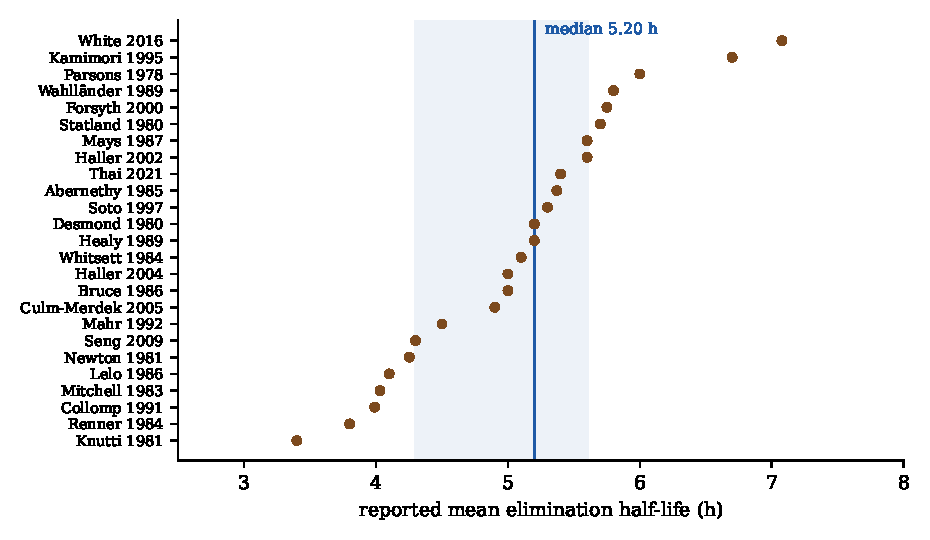
\includegraphics[width=0.92\linewidth]{fig/half_lives.pdf}
\caption{Mean elimination half-life reported for healthy adult control groups. Blue line: median;
shaded: interquartile range.}
\label{fig:hl}
\end{figure}

{\small
\begin{longtable}{p{0.17\linewidth}p{0.25\linewidth}p{0.3\linewidth}rr}
\caption{Half-life data (healthy adult control groups, oral caffeine).}\label{tab:hl}\\
\toprule
Study & Journal & Group & $t_{1/2}$ (h) & PMID \\
\midrule\endfirsthead
\toprule
Study & Journal & Group & $t_{1/2}$ (h) & PMID \\
\midrule\endhead
\halflifetable
\bottomrule
\end{longtable}}

\subsection{Volume of distribution and clearance}
The median of the volumes in Table~\ref{tab:v} is $V=\nVkg$\,L/kg. Together with $\ke$ this implies a
clearance of \nCLmodel\,mL/min/kg, in the middle of the values reported for healthy non-smokers
(Table~\ref{tab:cl}), which supports the internal consistency of the two parameters.

\begin{table}[H]
\centering\small
\begin{minipage}{0.48\linewidth}\centering
\caption{Volume of distribution.}\label{tab:v}
\begin{tabular}{p{0.68\linewidth}r}
\toprule Study & L/kg \\ \midrule
\voltable
\bottomrule
\end{tabular}
\end{minipage}\hfill
\begin{minipage}{0.48\linewidth}\centering
\caption{Reported clearance (model: \nCLmodel).}\label{tab:cl}
\begin{tabular}{p{0.68\linewidth}r}
\toprule Study & mL/min/kg \\ \midrule
\cltable
\bottomrule
\end{tabular}
\end{minipage}
\end{table}

\subsection{Absorption rate}
$\ka$ was chosen so that the model peaks at the median reported time to peak after drinks and solutions
(Table~\ref{tab:tmax}). Where a drink was sipped over several minutes (White 2016), time is counted from
the middle of drinking. The median is \nTmaxMed\,min, giving $\ka=\nKa$\,h$^{-1}$ (absorption half-time
about 9\,min). Peak concentrations were \emph{not} used for fitting, so they remain an independent check.

\begin{table}[H]
\centering\small
\caption{Time to peak used for $\ka$.}\label{tab:tmax}
\begin{tabular}{lr}
\toprule Study, condition & $t_{\max}$ (min) \\ \midrule
\tmaxtable
\bottomrule
\end{tabular}
\end{table}

\section{Validation}
\label{sec:valid}
Table~\ref{tab:valid} compares predicted with observed concentrations from studies whose concentrations
were not used to set any parameter. Landolt 1995 measured saliva; values were converted to plasma with the
saliva/plasma ratio of 0.74 (Newton 1981), and 70\,kg was assumed because weight was not reported.

\begin{table}[H]
\centering\small
\caption{Independent validation (mg/L plasma).}\label{tab:valid}
\begin{tabular}{p{0.55\linewidth}rrr}
\toprule Study & observed & predicted & ratio \\ \midrule
\validtable
\bottomrule
\end{tabular}
\end{table}

\begin{figure}[H]
\centering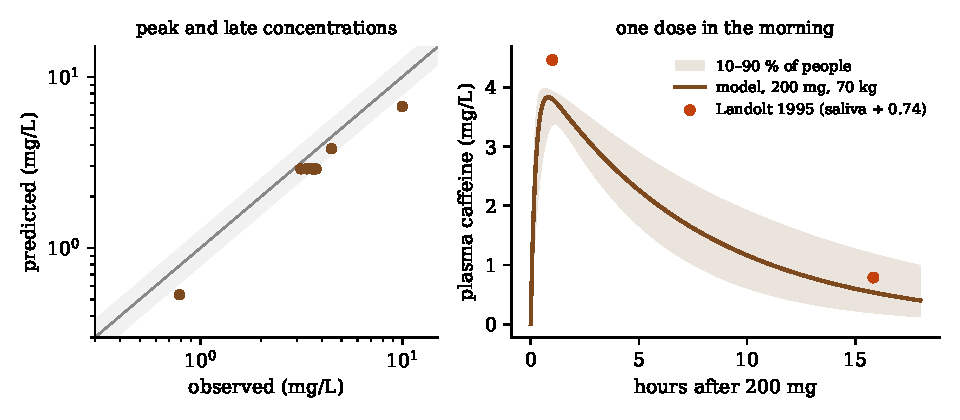
\includegraphics[width=0.95\linewidth]{fig/validation.pdf}
\caption{Left: predicted vs.\ observed concentrations (grey band: $\pm 25\,\%$). Right: model and
10--90\,\% population band after 200\,mg, with the two measurements of Landolt 1995.}
\label{fig:valid}
\end{figure}

\paragraph{Findings.} Prediction ratios range from \nRatioMin{} to \nRatioMax{} (median \nRatioMed).
\begin{itemize}
\item \emph{Peaks are about 20\,\% too low.} Studies report the mean of individual peaks, which is
higher than the peak of a typical person; simulating the population variability accounts for only about
1\,\% of the gap (factor \nPopPeakRatio). The rest is the early distribution phase that a one-compartment model omits:
just after absorption, caffeine has not yet spread through all body water, so blood levels are briefly
higher than the volume at steady state implies. The oral solution taken fasting (Blanchard 1983) was also
absorbed faster than drinks. Neither affects the amount in the body, which is what the application shows.
\item \emph{The late point (15.8\,h) is under-predicted by about a third.} The two measurements of
Landolt 1995 imply a half-life of about \nLandoltHalf\,h in that group, longer than the population median
but inside its spread; the point lies inside the 10--90\,\% band (Figure~\ref{fig:valid}).
\end{itemize}
The comparison supports the model shape and its order of magnitude; the individual uncertainty (next
section) is larger than the model error.

\section{What the application will show}
\label{sec:display}
\subsection{Milligrams in the body}
The main number is body$(t)$ summed over the user's entries: caffeine absorbed and not yet eliminated.
While a drink is still being absorbed (about the first hour), a small line can add ``+ X mg se ještě
vstřebává'' (gut$(t)$), so that a freshly logged drink does not seem to disappear. Figure~\ref{fig:single}
shows one small and one large energy drink: 150\,mg peaks at about 135\,mg in the body after
\nTmaxModel\,min and is below \nRefMg\,mg after about \nTRefOneFifty\,h.

\begin{figure}[H]
\centering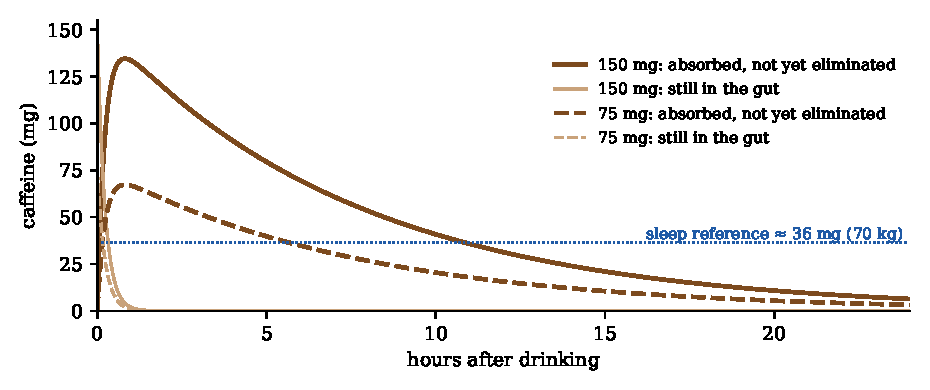
\includegraphics[width=0.92\linewidth]{fig/single_dose.pdf}
\caption{One large (150\,mg) and one small (75\,mg) energy drink.}
\label{fig:single}
\end{figure}

\subsection{Cups of coffee}
A ``cup of coffee'' is not a standard amount: espressos bought in coffee shops contained 48--317\,mg per
serving (Ludwig 2014) and up to 322\,mg (Crozier 2012). The sleep meta-analysis used 107\,mg per 250\,mL
cup (Gardiner 2023). The application uses a round \textbf{\nCupMg\,mg = 1 šálek} and should say so in
its explanation.

\subsection{Bedtime and the sleep reference}
\label{sec:sleep}
\paragraph{Evidence.} In a meta-analysis of 24 studies, caffeine reduced total sleep time by 45\,min and
sleep efficiency by 7\,\%, and lengthened sleep onset; to avoid a reduction in total sleep time, 107\,mg
(coffee) should be taken at least 8.8\,h before bed and 217.5\,mg (a pre-workout serving) at least 13.2\,h
before bed (Gardiner 2023). 400\,mg taken 6\,h before bed still disrupted sleep significantly in a
randomised home study (Drake 2013). In a laboratory study, 200\,mg at 07:10 still reduced sleep efficiency
and total sleep time at 23:00, when the saliva level was 3\,µmol/L (Landolt 1995).

\paragraph{Derivation.} Run through the model, Gardiner's two limits correspond to \nGCoffee{} and \nGPrew\,mg
still in the body at bedtime, and Landolt's measured level to \nLandoltMg\,mg at 70\,kg: three independent
routes that put the level from which sleep is measurably affected at roughly 35--40\,mg for a 70\,kg adult.
Drake's condition corresponds to \nDrakeMg\,mg, far above it, consistent with its clear effect
(Figure~\ref{fig:sleep}). We take the mean of the
two meta-analytic values, \textbf{\nRefMg\,mg at 70\,kg}, and scale it with body weight as
\textbf{\nRefMgKg\,mg/kg} (a plasma level of about \nRefConc\,mg/L), because the effect depends on the
concentration at the adenosine receptors, not on the amount.

\begin{figure}[H]
\centering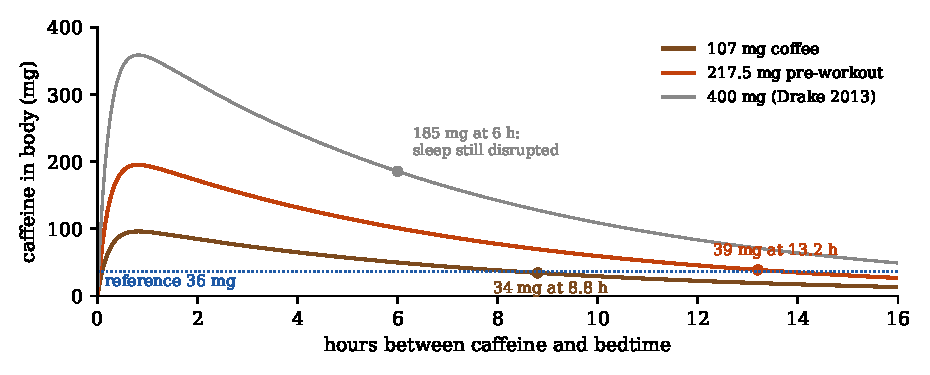
\includegraphics[width=0.92\linewidth]{fig/sleep_reference.pdf}
\caption{Caffeine in the body vs.\ hours before bedtime for the doses of Gardiner 2023 and Drake 2013.
Dots: the published limits run through the model.}
\label{fig:sleep}
\end{figure}

\paragraph{How to word it.} This is a \emph{soft} reference: it comes from average effects on total
sleep time; deep-sleep EEG changes were seen even near this level (Landolt 1995), and sensitivity to
caffeine varies with genetics (Nehlig 2018). The application should phrase it as ``\emph{kolem této
hodnoty a výš kofein podle studií v průměru zkracuje spánek; citlivější lidé to můžou cítit i při méně}'',
never as a safe limit.

\paragraph{Bedtime projection.} With a bedtime setting, the card shows body$(t_{\text{bed}})$ assuming no
further caffeine, and when the estimate falls below the reference. For a typical day of three energy
drinks (Figure~\ref{fig:day}), about \nDayBed\,mg would remain at 23:00 for a typical person
(10--90\,\%: \nDayBedLo--\nDayBedHi\,mg).

\begin{figure}[H]
\centering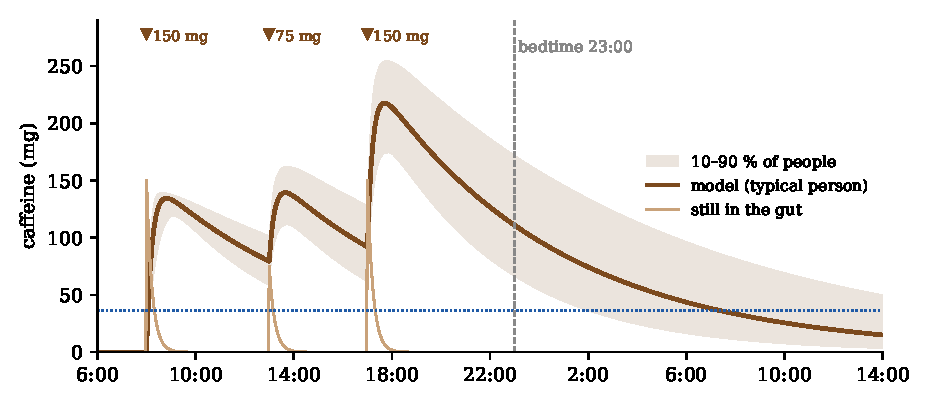
\includegraphics[width=0.92\linewidth]{fig/typical_day.pdf}
\caption{Large energy drink at 8:00, small at 13:00, large at 17:00. Dotted: sleep reference (70\,kg).
Band: 10--90\,\% of people (population variability of Seng 2009).}
\label{fig:day}
\end{figure}

\begin{figure}[H]
\centering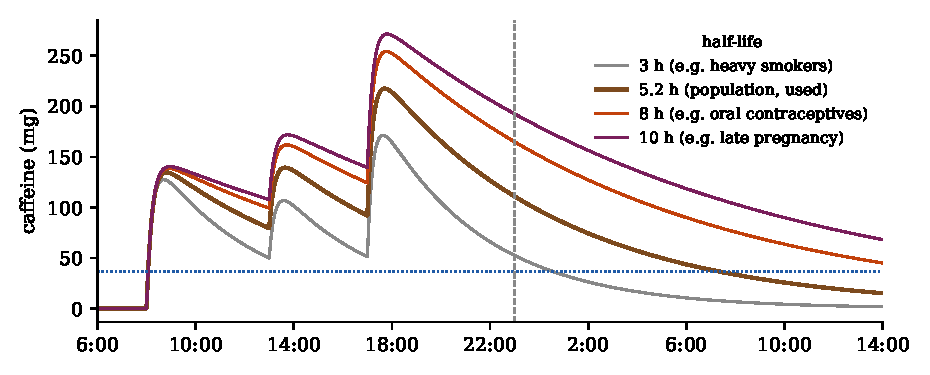
\includegraphics[width=0.92\linewidth]{fig/sensitivity.pdf}
\caption{Same day with other half-lives (option D, not used in version 1).}
\label{fig:sens}
\end{figure}

\section{Deployment specification (for later)}
\label{sec:deploy}
\begin{itemize}
\item \textbf{Code.} A new \texttt{src/lib/caffeinePk.ts} with the constants of
\texttt{ts\_constants.json} (written by \texttt{model.py}): \texttt{KA\_PER\_H} $=\nKa$,
\texttt{KE\_PER\_H} $=\nKe$, \texttt{V\_L\_PER\_KG} $=\nVkg$, \texttt{SLEEP\_REF\_MG\_PER\_KG} $=\nRefMgKg$,
\texttt{CUP\_MG} $=\nCupMg$; functions for body and gut amounts at a time, a curve for the chart, the amount
at bedtime and the time it falls below the reference (closed form for one dose, bisection for several,
like \texttt{pkTimesBelow} for kratom). Entries in the future (logged for later today) are ignored until
their time; entries older than 72\,h are ignored.
\item \textbf{Tests.} \texttt{caffeinePk.test.ts} pins the check values in \texttt{ts\_constants.json}
(e.g.\ 150\,mg: 133.5\,mg after 1\,h, 69.5\,mg after 6\,h, 31.2\,mg after 12\,h).
\item \textbf{Settings.} Body weight (default 70\,kg, e.g.\ 35--250\,kg) and bedtime (e.g.\ 23:00) in
\emph{Nastavení} when caffeine is selected; they need two new columns in \texttt{user\_settings} (one
migration), visible only to the owner.
\item \textbf{UI.} A card on the caffeine \emph{Dnes} page with the mg number, cups line, a chart of the last
24\,h plus a projection to the next morning with the bedtime line and the reference, and the honest
explanation (``Jak se to počítá?'').
\item \textbf{Privacy.} Computed in the browser from the user's own entries only; nothing new is stored or
shared. No notifications are planned.
\item \textbf{Changing the model} means editing \texttt{model.py}, re-running it, copying the constants
and re-running the tests, as for kratom.
\end{itemize}

\section{Limitations}
\begin{itemize}
\item One population half-life; real individuals differ by a factor of three or more
(10--90\,\%: \nTHalfTen--\nTHalfNinety\,h in the simulated population), most strongly with smoking,
oral contraceptives, pregnancy, liver disease and some medicines.
\item Linear kinetics; after very large doses or heavy daily intake, elimination may be slower than
assumed, so the estimate may then be too low.
\item Entries are user-reported; caffeine content of drinks varies widely (a ``cup'' is not a fixed amount).
\item Early peak concentrations are under-predicted; the displayed amount is not affected.
\item Tea, cola and chocolate count only if logged. Paraxanthine, which is also active, is not shown.
\item The sleep reference is an average effect on total sleep time from studies of mostly young healthy
adults and is not a safe limit.
\end{itemize}

\section*{References}
\small
\begin{enumerate}[leftmargin=*,label={}]
\item Abernethy DR, Todd EL (1985). Impairment of caffeine clearance by chronic use of low-dose oestrogen-containing oral contraceptives. \emph{Eur J Clin Pharmacol} 28:425--8. \pmid{4029248}.
\item Blanchard J, Sawers SJ (1983). The absolute bioavailability of caffeine in man. \emph{Eur J Clin Pharmacol} 24:93--8. \pmid{6832208}.
\item Bonati M, et al.\ (1982). Caffeine disposition after oral doses. \emph{Clin Pharmacol Ther} 32:98--106. \pmid{7083737}.
\item Cheng WS, et al.\ (1990). Dose-dependent pharmacokinetics of caffeine in humans: relevance as a test of quantitative liver function. \emph{Clin Pharmacol Ther} 47:516--24. \pmid{2328560}.
\item Crozier TW, et al.\ (2012). Espresso coffees, caffeine and chlorogenic acid intake: potential health implications. \emph{Food Funct} 3:30--3. \pmid{22130653}.
\item Denaro CP, et al.\ (1990). Dose-dependency of caffeine metabolism with repeated dosing. \emph{Clin Pharmacol Ther} 48:277--85. \pmid{2401126}.
\item Drake C, et al.\ (2013). Caffeine effects on sleep taken 0, 3, or 6 hours before going to bed. \emph{J Clin Sleep Med} 9:1195--200. \pmid{24235903}.
\item Faber MS, Fuhr U (2004). Time response of cytochrome P450 1A2 activity on cessation of heavy smoking. \emph{Clin Pharmacol Ther} 76:178--84. \pmid{15289794}.
\item Fendt R, et al.\ (2021). Data-driven personalization of a physiologically based pharmacokinetic model for caffeine: a systematic assessment. \emph{CPT Pharmacometrics Syst Pharmacol} 10:782--793. \pmid{34053199}.
\item Gardiner C, et al.\ (2023). The effect of caffeine on subsequent sleep: a systematic review and meta-analysis. \emph{Sleep Med Rev} 69:101764. \pmid{36870101}.
\item Grzegorzewski J, et al.\ (2021). Pharmacokinetics of caffeine: a systematic analysis of reported data for application in metabolic phenotyping and liver function testing. \emph{Front Pharmacol} 12:752826. \pmid{35280254}.
\item Haller CA, et al.\ (2004). Enhanced stimulant and metabolic effects of combined ephedrine and caffeine. \emph{Clin Pharmacol Ther} 75:259--73. \pmid{15060505}.
\item Jeppesen U, et al.\ (1996). A fluvoxamine--caffeine interaction study. \emph{Pharmacogenetics} 6:213--22. \pmid{8807660}.
\item Kaplan GB, et al.\ (1997). Dose-dependent pharmacokinetics and psychomotor effects of caffeine in humans. \emph{J Clin Pharmacol} 37:693--703. \pmid{9378841}.
\item Knutti R, et al.\ (1981). Effect of pregnancy on the pharmacokinetics of caffeine. \emph{Eur J Clin Pharmacol} 21:121--6. \pmid{7341280}.
\item Landolt HP, et al.\ (1995). Caffeine intake (200 mg) in the morning affects human sleep and EEG power spectra at night. \emph{Brain Res} 675:67--74. \pmid{7796154}.
\item Lelo A, et al.\ (1986). Comparative pharmacokinetics of caffeine and its primary demethylated metabolites paraxanthine, theobromine and theophylline in man. \emph{Br J Clin Pharmacol} 22:177--82. \pmid{3756065}.
\item Liguori A, et al.\ (1997). Absorption and subjective effects of caffeine from coffee, cola and capsules. \emph{Pharmacol Biochem Behav} 58:721--6. \pmid{9329065}.
\item Ludwig IA, et al.\ (2014). Variations in caffeine and chlorogenic acid contents of coffees: what are we drinking? \emph{Food Funct} 5:1718--26. \pmid{25014672}.
\item Mahr G, et al.\ (1992). Effects of temafloxacin and ciprofloxacin on the pharmacokinetics of caffeine. \emph{Clin Pharmacokinet} 22 Suppl 1:90--7. \pmid{1319876}.
\item Nehlig A (2018). Interindividual differences in caffeine metabolism and factors driving caffeine consumption. \emph{Pharmacol Rev} 70:384--411. \pmid{29514871}.
\item Newton R, et al.\ (1981). Plasma and salivary pharmacokinetics of caffeine in man. \emph{Eur J Clin Pharmacol} 21:45--52. \pmid{7333346}.
\item Parsons WD, Neims AH (1978). Effect of smoking on caffeine clearance. \emph{Clin Pharmacol Ther} 24:40--5. \pmid{657717}.
\item Seng KY, et al.\ (2009). Population pharmacokinetics of caffeine in healthy male adults using mixed-effects models. \emph{J Clin Pharm Ther} 34:103--14. \pmid{19125908}.
\item Thai C, et al.\ (2021). A phase 1 open-label, fixed-sequence pharmacokinetic drug interaction trial to investigate the effect of cannabidiol on the CYP1A2 probe caffeine in healthy subjects. \emph{Clin Pharmacol Drug Dev} 10:1279--1289. \pmid{33951339}.
\item White JR Jr, et al.\ (2016). Pharmacokinetic analysis and comparison of caffeine administered rapidly or slowly in coffee chilled or hot versus chilled energy drink in healthy young adults. \emph{Clin Toxicol} 54:308--12. \pmid{27100333}.
\item Studies contributing only a half-life value are listed with their PMID in Table~\ref{tab:hl}.
\end{enumerate}
\end{document}
